\documentclass[12pt,t]{beamer}
% \documentclass[t]{beamer}
\usepackage[utf8]{inputenc}
\usepackage[catalan]{babel}
\usepackage{hyperref}
\usepackage{amsfonts,amssymb,amsmath,amsthm, wasysym}
\usepackage[T1]{fontenc}        
\usepackage{pgf}
\usepackage{pgfpages}
%\usepackage{tikz}
%\usetikzlibrary{arrows,shapes,plotmarks,backgrounds,trees,positioning}
%\usetikzlibrary{decorations.pathmorphing,calc,snakes}
%\usepackage{marvosym}
%
\usetheme[hideothersubsections,left]{Marburg}
\usecolortheme{sidebartab}
\useinnertheme[shadow]{rounded}
% \useoutertheme[footline=empty,subsection=true,compress]{infolines}
% \useoutertheme[footline=empty,subsection=true,compress]{miniframes}
% \usefonttheme{serif}

\setbeamertemplate{caption}[numbered]
\setbeamertemplate{navigation symbols}{}


\newcommand{\red}[1]{\textcolor{red}{#1}}
\newcommand{\green}[1]{\textcolor{green}{#1}}
\newcommand{\blue}[1]{\textcolor{blue}{#1}}
\newcommand{\gray}[1]{\textcolor{gray}{#1}}
\renewcommand{\emph}[1]{{\color{red}#1}}

\setbeamertemplate{frametitle}
{\begin{centering}
\medskip
\color{blue}
\textbf{\insertframetitle}
\medskip
\end{centering}
}
\usecolortheme{rose}
\usecolortheme{dolphin}
\mode<presentation>

\usepackage{listings}

\lstset{
language=R, %
aboveskip=1 ex, %
belowskip=-4ex, %
linewidth=\textwidth,
%xleftmargin=0.5cm,
%xrightmargin=0.5cm,
basicstyle={\footnotesize\ttfamily}, %
commentstyle=\ttfamily\color{red}, %
numbers=none, %
numberstyle=\ttfamily\color{gray}\footnotesize,
stepnumber=1,
numbersep=5pt,
backgroundcolor=\color{gray!20},%15
showspaces=false,
%showstringspaces=false,
showtabs=false,
frame=single, %????
framerule=0pt,
keepspaces=true,
tabsize=2,
captionpos=b, %
breaklines=true, %
breakatwhitespace=false,  %
showstringspaces=false,
title=\lstname,
literate={{á}{{\'a}}1 {é}{{\'e}}1 {í}{{\'i}}1 {ó}{{\'o}}1 {ú}{{\'u}}1
  {Á}{{\'A}}1 {É}{{\'E}}1 {Í}{{\'I}}1 {Ó}{{\'O}}1 {Ú}{{\'U}}1
  {à}{{\`a}}1 {è}{{\`e}}1 {ì}{{\`i}}1 {ò}{{\`o}}1 {ù}{{\`u}}1
  {À}{{\`A}}1 {È}{{\'E}}1 {Ì}{{\`I}}1 {Ò}{{\`O}}1 {Ù}{{\`U}}1
  {ä}{{\"a}}1 {ë}{{\"e}}1 {ï}{{\"i}}1 {ö}{{\"o}}1 {ü}{{\"u}}1
  {Ä}{{\"A}}1 {Ë}{{\"E}}1 {Ï}{{\"I}}1 {Ö}{{\"O}}1 {Ü}{{\"U}}1 {ñ}{{\~n}}1 {Ñ}{{\~N}}1
  {â}{{\^a}}1 {ê}{{\^e}}1 {î}{{\^i}}1 {ô}{{\^o}}1 {û}{{\^u}}1
  {Â}{{\^A}}1 {Ê}{{\^E}}1 {Î}{{\^I}}1 {Ô}{{\^O}}1 {Û}{{\^U}}1
  {œ}{{\oe}}1 {Œ}{{\OE}}1 {æ}{{\ae}}1 {Æ}{{\AE}}1 {ß}{{\ss}}1
  {ç}{{\c c}}1 {Ç}{{\c C}}1 {ø}{{\o}}1 {å}{{\r a}}1 {Å}{{\r A}}1
  {€}{{\EUR}}1 {£}{{\pounds}}1 {¡}{{\textexclamdown}}1 {¿}{{\textquestiondown}}1 {!}{{!}}1
  {·}{{\textperiodcentered}}1}
 }
\lstdefinestyle{petit}{basicstyle={\scriptsize\ttfamily}}

\newcommand{\CC}{\mathbb{C}}
\newcommand{\RR}{\mathbb{R}}
\newcommand{\ZZ}{\mathbb{Z}}
\newcommand{\NN}{\mathbb{N}}
\newcommand{\KK}{\mathbb{K}}
\newcommand{\MM}{\mathcal{M}}
%\newcommand{\dbinom}{\displaystyle\binom}

\newcommand{\limn}{{\displaystyle \lim_{n\to\infty}}}
\renewcommand{\leq}{\leqslant}
\renewcommand{\geq}{\geqslant}
\def\tendeix{{\displaystyle\mathop{\Longrightarrow }_{\scriptscriptstyle
n\to\infty}}}

\newcommand{\matriu}[1]{\left(\begin{matrix} #1 \end{matrix}\r\right)}

% \newcommand{\qed}{\hbox{}\nobreak\hfill\vrule width 1.4mm he\right 1.4mm depth 0mm
%     \par \goodbreak \smallskip}
%
% %
\theoremstyle{plain}
\newtheorem{teorema}{Teorema}
\newtheorem{prop}{Proposició}
\newtheorem{cor}{Coro\l.lari}
\theoremstyle{definition}
\newtheorem{exemple}{Exemple}
\newtheorem{defin}{Definició}
\newtheorem{obs}{Observació}

\newcounter{seccions}
\newcommand{\seccio}[1]{\addtocounter{seccions}{1}
\medskip\par\noindent\emph{\theseccions.
#1}\smallskip\par }

\newcommand{\EM}{\Omega}
\newcommand{\PP}{\mathcal{P}}

\title[\red{Bioestadística}]{}
\author[]{Cesc Rosselló}
\date{}

\addtobeamertemplate{frametitle}{}{\vspace*{-1ex}}

\begin{document}
\beamertemplatedotitem



\begin{frame}
\vfill
\begin{center}
\gray{\LARGE Regresión lineal simple}
\end{center}
\vfill
\end{frame}



\section{Regresión lineal simple}
\subsection{Problema básico}

\begin{frame}
\frametitle{Problema básico}

La tabla siguiente nos da las alturas (en cm) y el VEF (en litros) de 20 estudiantes varones\medskip

\begin{center}
\begin{tabular}{cc|cc|cc}
Altura & VEF & Altura & VEF &Altura & VEF \\\hline
164.0 & 3.54 & 172.0 & 3.78 & 178.0 & 2.98\\
167.0 & 3.54 & 174.0 & 4.32 & 180.7 & 4.80\\
170.4 & 3.19 & 176.0 & 3.75 & 181.0 & 3.96\\
171.2 & 2.85 & 177.0 & 3.09 & 183.1 & 4.78\\
171.2 & 3.42 & 177.0 & 4.05 & 183.6 & 4.56\\
171.3 & 3.20 & 177.0 & 5.43 & 183.7 & 4.68\\
172.0 & 3.60 & 177.4 & 3.60
\end{tabular}
\end{center}
\end{frame}



\begin{frame}
\frametitle{Problema básico}
\vspace*{-1cm}

\begin{center}
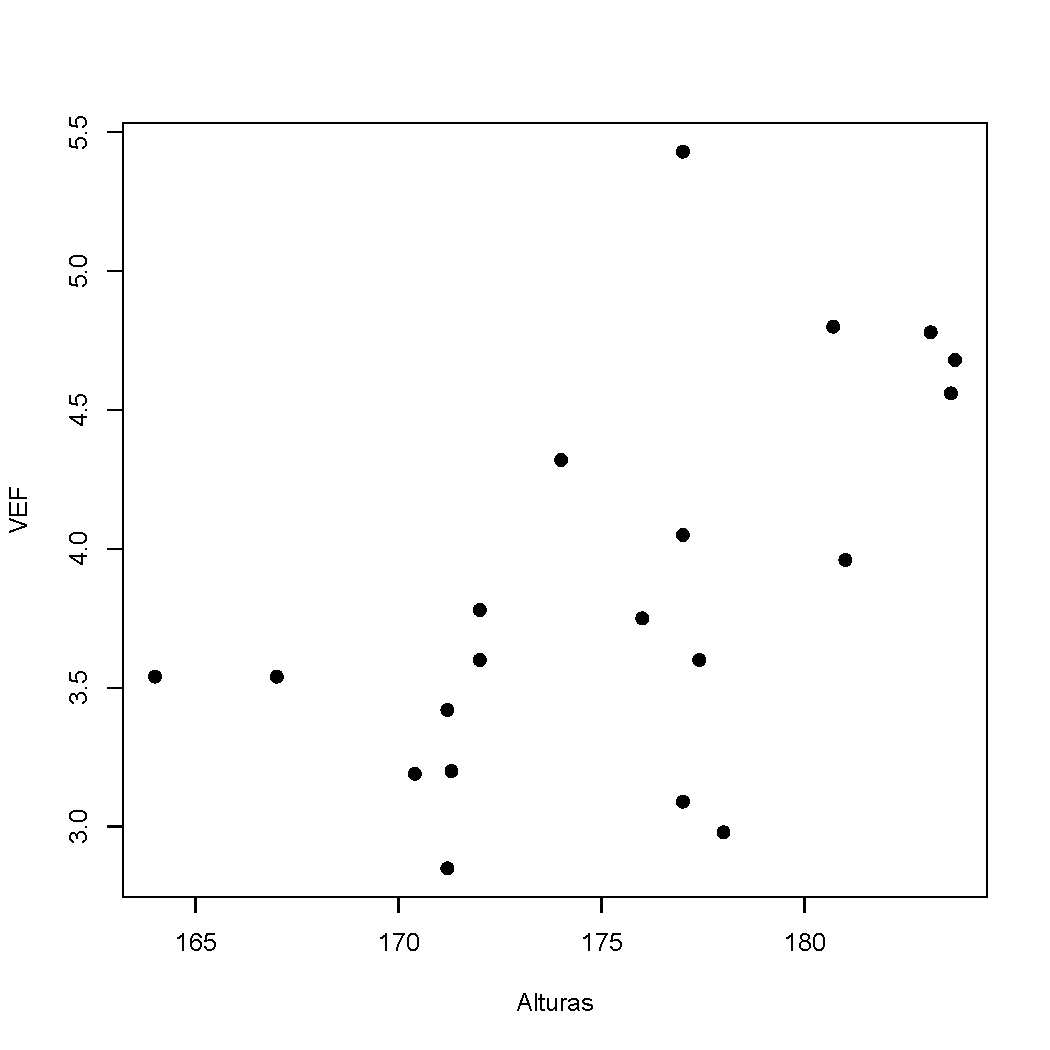
\includegraphics[width=0.8\linewidth]{plotVEF1.pdf}
\end{center}
\end{frame}


\begin{frame}
\frametitle{Problema básico}
\vspace*{-1cm}

\begin{center}
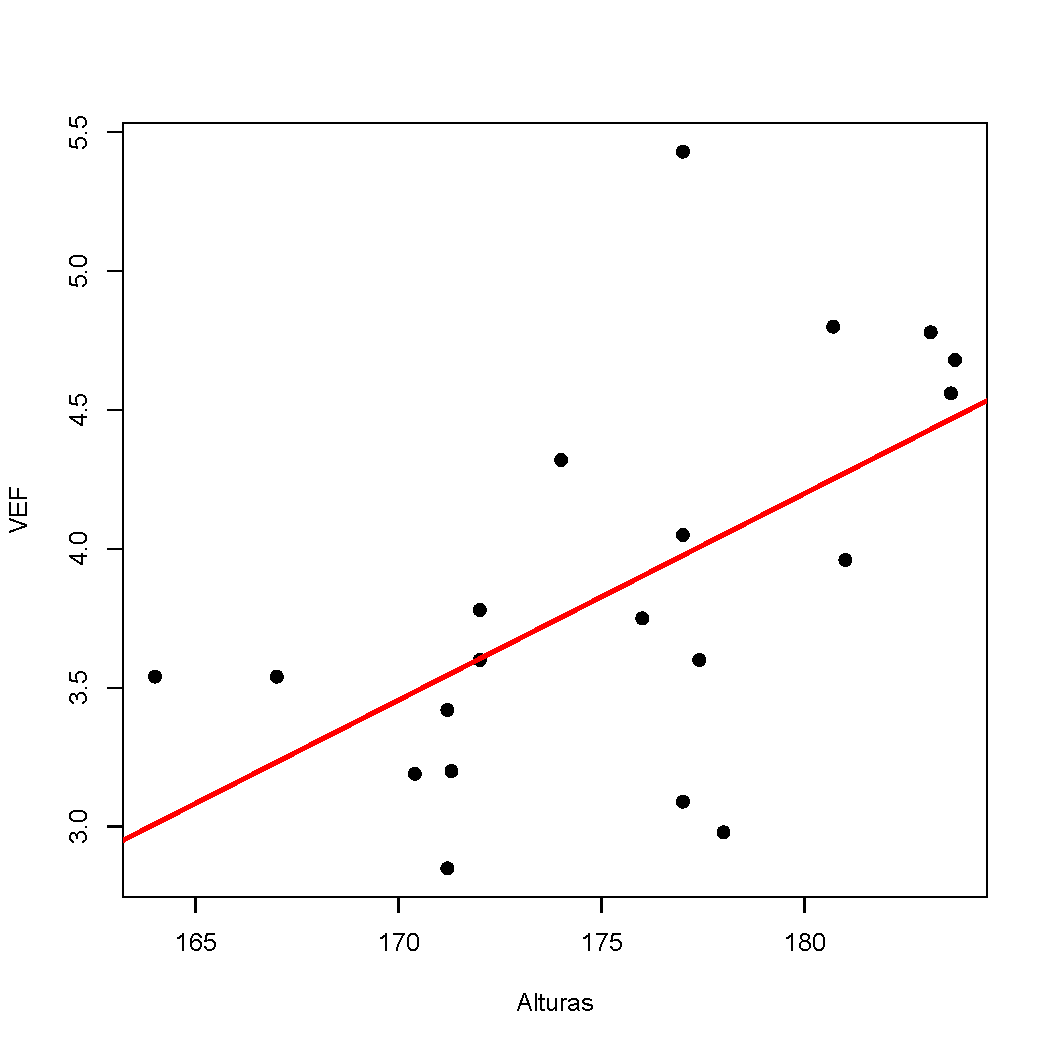
\includegraphics[width=0.8\linewidth]{plotVEF2.pdf}
\end{center}
\end{frame}




\begin{frame}
\frametitle{Problema básico}

Tenemos pares de observaciones de dos variables $X,Y$:
$$
(x_i,y_i)_{i=1,2,\ldots,n}
$$

\begin{itemize}
\item La variable (no necesariamente aleatoria) $X$ es la variable  \emph{independiente}

\item La variable aleatoria $Y$ es la variable \emph{dependiente}
\end{itemize}
\medskip

Queremos encontrar la \emph{relación lineal}  
$$
Y=b_0+b_1X
$$
que mejor explique los valores de $Y$ en función de  los de $X$
\end{frame}

\begin{frame}
\frametitle{Regresión lineal simple}

Suponemos que (en la vida real)
$$
\mu_{Y|x}=\beta_0+\beta_1 x
$$
donde
\begin{itemize}
\item \red{$Y|x$} es la v.a.\ $Y$ restringida a los individuos en los que $X$ vale $x$\medskip

\item \red{$\mu_{Y|x}$} es el valor esperado de $Y$ cuando $X$ vale $x$\medskip

\item \red{$\beta_0$} (\emph{término independiente}) y \red{$\beta_1$} (\emph{pendiente}) son 
parámetros que queremos estimar 
\end{itemize}\bigskip

(Porque\ldots\ si no creemos que esta relación existe, ¿para qué vamos a buscar una expresión de $Y$ lineal en $X$?)

\end{frame}

\begin{frame}
\frametitle{Regresión lineal simple}

Con una muestra $(x_i,y_i)_{i=1,\ldots,n}$, calcularemos estimaciones \red{$b_0$} y \red{$b_1$} de $\beta_0$
y  $\beta_1$
\medskip

Esto nos dará la \emph{recta de regresión} para nuestra muestra:
$$
\red{\widehat{y}=b_0+b_1 x}
$$
Esta recta sirve, por ejemplo, para, dado un valor $x_0$ de $X$, estimar el valor (esperado) 
$$
\red{\widehat{y}_0=b_0+b_1 x_0}
$$ 
de $Y$ sobre un individuo para el que $X$ valga $x_0$
\end{frame}

\subsection{Mínimos cuadrados}

\begin{frame}
\frametitle{Mínimos cuadrados}

Dados $b_0,b_1$, el \red{residuo}, o \red{error}, \red{$i$-ésimo} del modelo $\widehat{y}=b_0+b_1 x$ es
$$
\red{e_i}=y_i-b_0-b_1 x_i
$$
\begin{center}
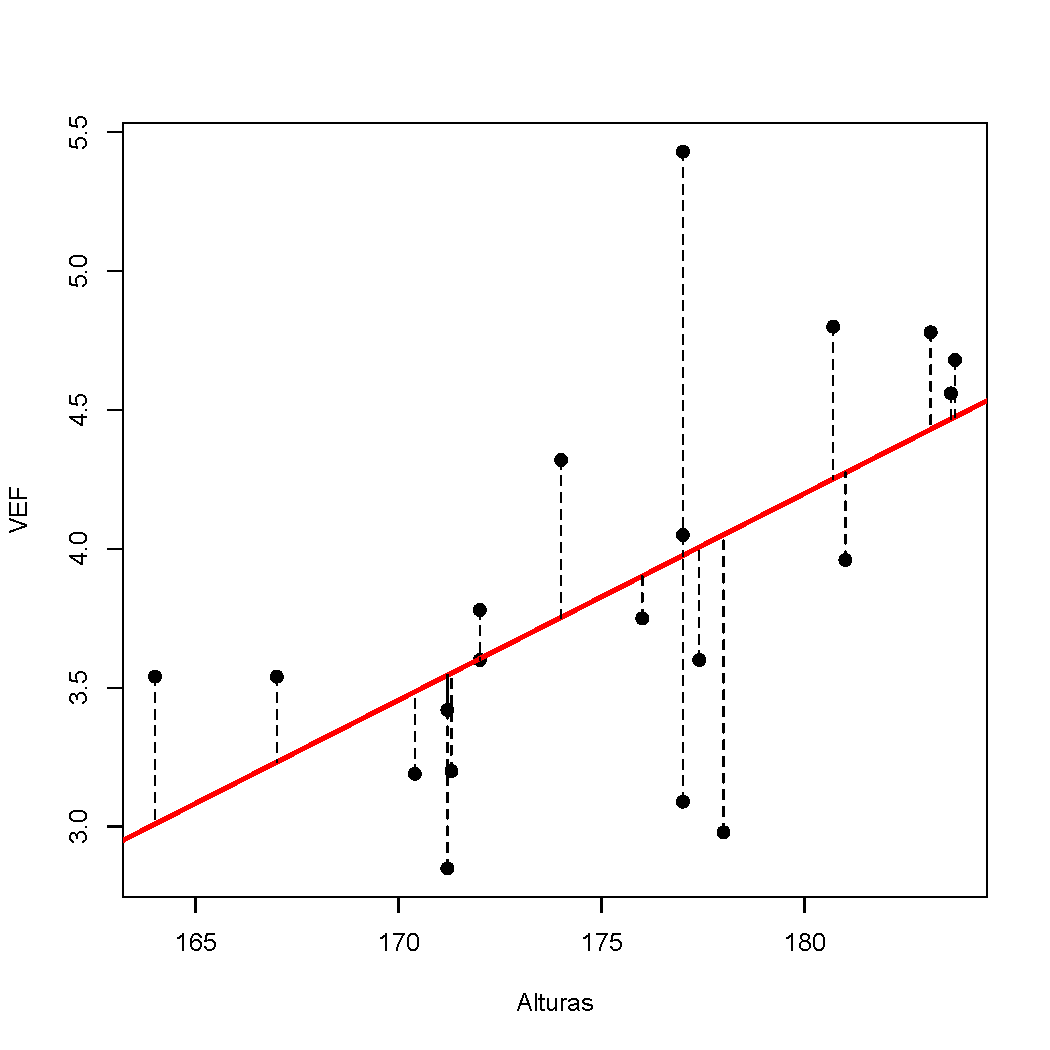
\includegraphics[width=0.6\linewidth]{plotVEF3.pdf}
\end{center}

\end{frame}

\begin{frame}
\frametitle{Mínimos cuadrados}


Los \red{estimadores por mínimos cuadrados de $\beta_0$ y $\beta_1$} son los valores $b_0,b_1$ que minimizan la suma de los cuadrados de los errores: es decir, tales que
$$
\sum_{i=1}^n (y_i-b_0-b_1 x_i)^2\qquad \mbox{sea mínimo}
$$
Derivando, igualando a 0, operando etc. obtenemos

\begin{teorema}
Los estimadores por mínimos cuadrados $b_0$ y $b_1$ de $\beta_0$ y $\beta_1$ son
$$
b_1 =\frac{\widetilde{s}_{xy}}{\widetilde{s}^{\, 2}_x},\quad b_0 = \overline{y}-b_1 \overline{x}
$$
\end{teorema}

\end{frame}

\begin{frame}[fragile]
\frametitle{Mínimos cuadrados}

La recta de regresión por mínimos cuadrados de $Y$ en función de $X$ se calcula con \red{\tt lm(y\~{}x)}\medskip

Sus coeficientes $b_0$ y $b_1$ son \red{\tt lm(y\~{}x)\$coefficients}\medskip

\begin{lstlisting}
> Alturas=c(164.0,167.0,170.4,171.2,171.2, 171.3,172.0,172.0,174.0,176.0,177.0, 177.0,177.0,177.4,178.0,180.7,181.0, 183.1,183.6,183.7)
> VEF=c(3.54,3.54,3.19,2.85,3.42,3.20,3.78, 3.60,4.32,3.75,3.09,4.05,5.43,3.60, 2.98,4.80,3.96,4.78,4.56,4.68)
> lm(VEF~Alturas)$coefficients
(Intercept)     Alturas 
-9.19038879  0.07438926 
\end{lstlisting}
Obtenemos la recta
$$
\widehat{\mbox{VEF}}=-9.1904+  0.0744\cdot \mbox{Alturas}
$$
\end{frame}

\begin{frame}[fragile]
\frametitle{Mínimos cuadrados}
Comprobemos el teorema\medskip

\begin{lstlisting}
> lm(VEF~Alturas)$coefficients
(Intercept)     Alturas 
-9.19038879  0.07438926 
> b1=cov(Alturas,VEF)/var(Alturas)
> b1
[1] 0.07438926
> b0=mean(VEF)-b0*mean(Alturas)
> b0
[1] -9.190389
\end{lstlisting}\medskip

¿Qué VEF esperamos en un estudiante de 175 cm?
\begin{lstlisting}
> round(b0+b1*175,2)
[1] 3.83
\end{lstlisting}


\end{frame}


\begin{frame} 
\frametitle{¡Cuidado!}

Los cálculos involucrados en la regresión lineal son muy poco robustos: los redondeos
pueden influir mucho en el resultado final
\bigskip

En \blue{\url{http://en.wikipedia.org/wiki/simple_linear_regression}} encontraréis un ejemplo detallado de una regresión de peso en función de altura
\medskip

Si la calculamos en pulgadas y la pasamos a metros redondeando a cm da 
$$
\widehat{y}=61.675x-39.746
$$
Si primero traducimos las pulgadas a metros redondeando a cm y calculamos la recta de regresión, da
$$
\widehat{y}=61.272x-39.062
$$




\end{frame}


\begin{frame}
\frametitle{Propiedades}

\begin{itemize}
\item La recta de regresión pasa por el par de medias muestrales 
$(\overline{x},\overline{y})$:
$$
b_0+b_1 \overline{x}=\overline{y}
$$

\item La media de los valores estimados es igual a la media de los
observados:
$$
\overline{\,\widehat{y}\,} = \overline{y}
$$
\end{itemize}

\end{frame}

\subsection{Coef. de determinación}%%%%
\begin{frame}
\frametitle{Coeficiente de determinación}

Siguiendo la filosofía ANOVA, entendemos que  $\widehat{y}=b_0+b_1x$ es una buena aproximación de $y$ como función lineal de $x$ cuando la variabilidad de $\widehat{y}$ explica mucha parte de la variabilidad de $y$\bigskip

Se cuantifica con el \emph{coeficiente de determinación $R^2$}. Con R se calcula con
\red{\tt summary(lm(y\~{}x))\$r.squared}\bigskip

$R^2$ toma valores entre 0 y 1, y cuánto más se acerca a 1, mayor se considera el ajuste de la recta de regresión a la muestra

\end{frame}

\begin{frame}[fragile]
\frametitle{Coeficiente de determinación}

\begin{lstlisting}
> plot(Datos,pch=19)
> abline(lm(VEF~Alturas), col="red")
\end{lstlisting}\vspace*{-3ex}

\begin{center}
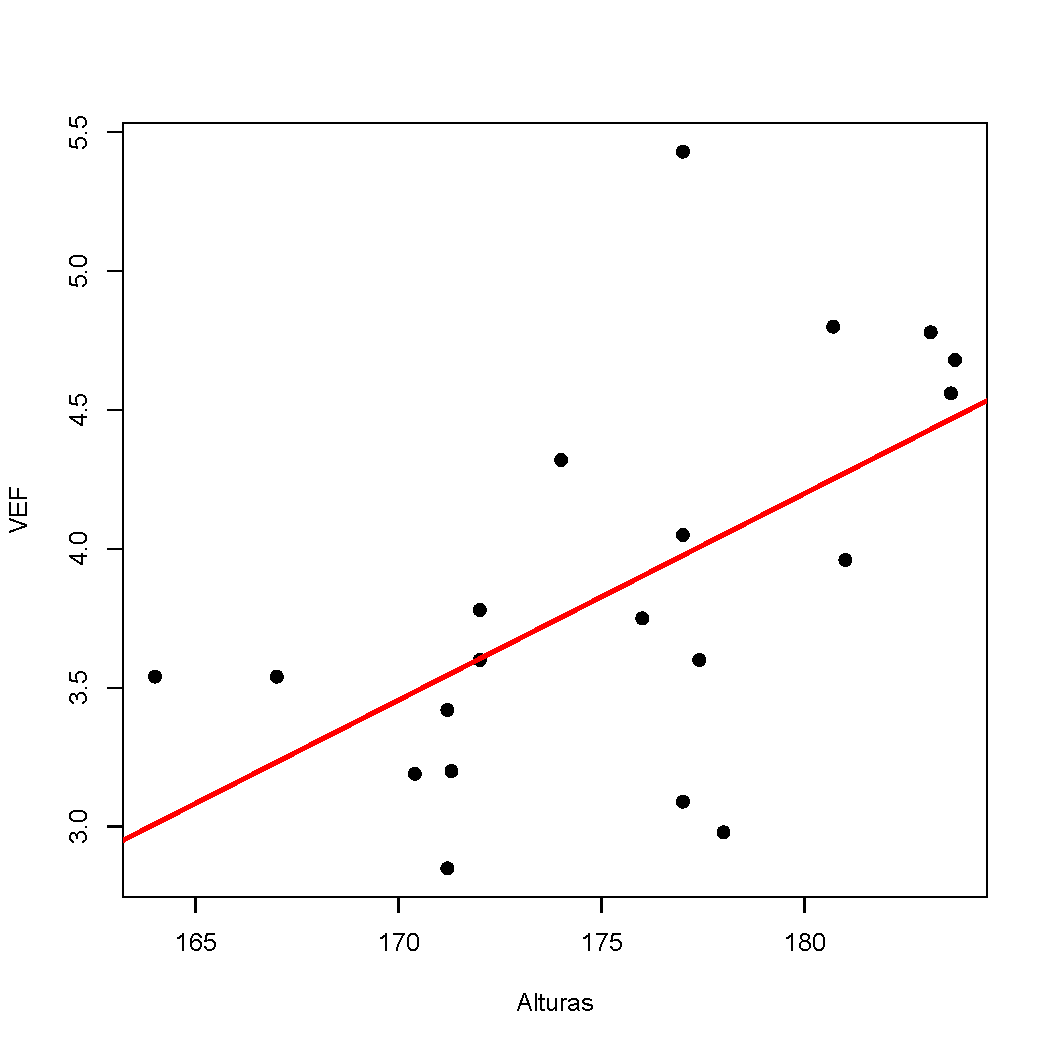
\includegraphics[width=0.6\linewidth]{plotVEF2.pdf}
\end{center}\vspace*{-3ex}


\begin{lstlisting}
> summary(lm(VEF~Alturas))$r.squared
[1] 0.3379069
\end{lstlisting}

\end{frame}

\begin{frame}
\frametitle{Coeficiente de determinación}
Sean:
\begin{itemize}
\item $\red{SS_T} =\sum\limits_{i=1}^n(y_i-\overline{y})^2=(n-1)\cdot \widetilde{s}_y^2$: \red{suma total de cuadrados}

\item $\red{SS_R}=\sum\limits_{i=1}^n(\widehat{y}_i-\overline{y})^2=(n-1)\cdot \widetilde{s}_{\widehat{y}}^2$: \red{suma de cuadrados de la regresión} 

\item $\red{SS_E}=\sum\limits_{i=1}^n e_i^2$: \red{suma de cuadrados de los errores}
\end{itemize}

\begin{teorema}
En una regresión lineal por mínimos cuadrados, se tiene que
$$
SS_T=SS_R+SS_E
$$
\end{teorema}

\end{frame}

\begin{frame}
\frametitle{Coeficiente de determinación}
El \emph{coeficiente de determinación} de una regresión lineal es
$$
\red{R^2}=\frac{SS_R}{SS_T}=\frac{\widetilde{s}_{\widehat{y}}^2}{\widetilde{s}_y^2}
$$
Por lo tanto, $R^2$ es la fracción de la varianza de $y$ que queda explicada por la varianza de $\widehat{y}$\medskip

Además, operando, se tiene:
\begin{teorema}
En una regresión lineal por mínimos cuadrados, \red{$R^2=r_{xy}^2$}
\end{teorema}\medskip

Cuánto más se acerca $R^2$ (y por lo tanto $r_{xy}$) a 1, más se acercan los puntos $(x_i,y_i)$ a una recta: la de regresión
\end{frame}

\begin{frame}[fragile]
\frametitle{¡Cuidado!}
No es conveniente valorar la bondad del modelo solo con el valor de $R^2$. Añadid un gráfico.\medskip

Considerad los cuatro conjuntos de pares $(x_i,y_i)_{i=1,\ldots,11}$ contenidos en el  dataframe \texttt{anscombe} de R:
\begin{lstlisting}
> str(anscombe)
'data.frame':	11 obs. of 8 variables:
$ x1: num 10 8 13 9 11 14 6 4 12 7 ...
$ x2: num 10 8 13 9 11 14 6 4 12 7 ...
$ x3: num 10 8 13 9 11 14 6 4 12 7 ...
$ x4: num 8 8 8 8 8 8 8 19 8 8 ...
$ y1: num 8.04 6.95 7.58 8.81 8.33 ...
$ y2: num 9.14 8.14 8.74 8.77 9.26 8.1 6.13 3.1 ...
$ y3: num 7.46 6.77 12.74 7.11 7.81 ...
$ y4: num 6.58 5.76 7.71 8.84 8.47 7.04 5.25 12.5 ...
\end{lstlisting}

\end{frame}

\begin{frame}[fragile]
\frametitle{¡Cuidado!}
Calculemos los $R^2$ de las regresiones\medskip

\begin{lstlisting}
> summary(lm(y1~x1,data=anscombe))$r.squared
[1] 0.6665425
> summary(lm(y2~x2,data=anscombe))$r.squared
[1] 0.6665425
> summary(lm(y3~x3,data=anscombe))$r.squared
[1] 0.6665425
> summary(lm(y4~x4,data=anscombe))$r.squared
[1] 0.6665425
\end{lstlisting}\medskip

%> #Vamos a representar los resultados
%> par(mfrow=c(2,2))
%> plot(y1~x1,data=anscombe)
%> abline(lm(y1~x1,data=anscombe),col=2)
%> plot(y2~x2,data=anscombe)
%> abline(lm(y2~x2,data=anscombe),col=2)
%> plot(y3~x3,data=anscombe)
%> abline(lm(y3~x3,data=anscombe),col=2)
%> plot(y4~x4,data=anscombe)
%> abline(lm(y4~x4,data=anscombe),col=2)
\end{frame}

\begin{frame}
\frametitle{¡Cuidado!}

Pero los cuatro gráficos son:\vspace*{-2ex}

\begin{center}
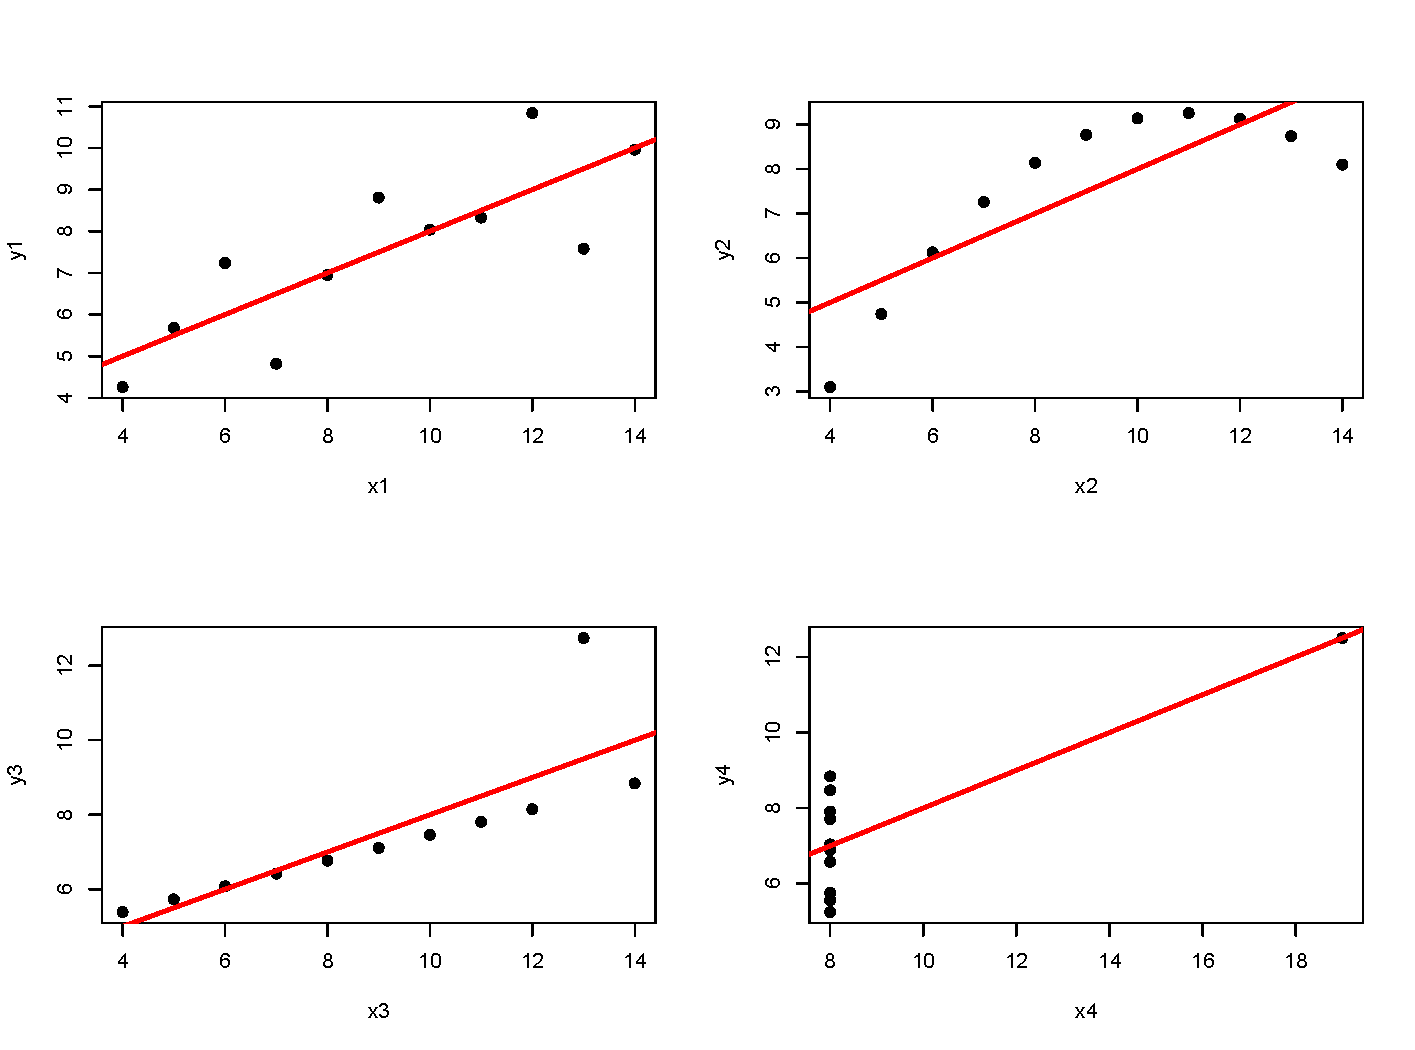
\includegraphics[width=\linewidth]{mismo_r2.pdf}
\end{center}

\end{frame}

%%%%%%%%%%%%%%%%%%%%


\subsection{Int. de confianza}

\begin{frame}
\frametitle{Más propiedades}

Si todas las vv.aa.\ \red{error}, o \red{residuo},
$$
\red{E_{x_i}}=(Y|x_i)-\beta_0-\beta_1 x_i
$$
son normales de media 0 y la misma varianza, e incorreladas dos a dos:\medskip

\begin{itemize}
\item $E(b_0)=\beta_0$ y $E(b_1)=\beta_1$\medskip

\item Entre todos los estimadores \red{insesgados} de $\beta_0$ y $\beta_1$, $b_0$ y $b_1$ son los que tienen menor error estándar\medskip

\item (Unos estadísticos relacionados con) $b_0$ y $b_1$ tienen distribuciones conocidas, que permiten calcular intervalos de confianza para $\beta_0$, $\beta_1$ y $\mu_{Y|x_0}$ usando la t de Student
\end{itemize}

\end{frame}




\begin{frame}[fragile]
\frametitle{Con R obtenemos mucha información}

\begin{lstlisting}[style=petit]
> summary(lm(VEF~Alturas))

Call:
lm(formula = VEF ~ Alturas)

Residuals:
     Min       1Q   Median       3Q      Max 
-1.07090 -0.32367  0.03446  0.31797  1.45349 

Coefficients:
            Estimate Std. Error t value Pr(>|t|)   
(Intercept) -9.19039    4.30644  -2.134  0.04684 * 
Alturas      0.07439    0.02454   3.031  0.00719 **
---
Signif. codes:  0 `***' 0.001 `**' 0.01 `*' 0.05 `.' 0.1 ` ' 1

Residual standard error: 0.5892 on 18 degrees of freedom
Multiple R-squared: 0.3379, Adjusted R-squared: 0.3011 
F-statistic: 9.187 on 1 and 18 DF,  p-value: 0.007185
\end{lstlisting}

\end{frame}


\begin{frame}
\frametitle{¿Tiene sentido una regresión lineal?}

Si $\beta_1=0$,  el modelo de regresión lineal no tiene sentido: significa que $\mu_{Y|x}=b_0$ para todo $x$, es decir, que $Y$ no depende de $X$\medskip

El p-valor del contraste 
$$
\left\{\begin{array}{l}
H_0:\beta_1=0\\
H_1:\beta_1 \neq 0
\end{array}
\right.
$$
es el valor de la columna \texttt{Pr(>|t|)} y fila correspondiente a la variable independiente (y, para la regresión lineal simple, también el \texttt{p-value} de la última fila)\medskip

En el ejemplo anterior vale 0.007185, lo que nos permite concluir que $\beta_1 \neq 0$



\end{frame}




\begin{frame}[fragile]
\frametitle{Intervalos de confianza}
Los IC 95\% para $\beta_0$ y $\beta_1$ se obtienen con la función \red{\tt confint(lm(y\~{}x))}\medskip

\begin{lstlisting}
> confint(lm(VEF~Alturas))
                   2.5 %     97.5 %
(Intercept) -18.23788410 -0.1428935
Alturas       0.02282546  0.1259531
\end{lstlisting}

Con el IC 95\% de $\beta_1$ también podemos contrastar si $\beta_1=0$ o no\medskip

En este caso, el IC 95\% va de 0.023 a 0.126, no contiene el 0
\end{frame}



\begin{frame}[fragile]
\frametitle{Intervalos de confianza}
El IC 95\% para $\mu_{Y|x_0}$ se obtiene con la construcción siguiente:\medskip

\begin{lstlisting}
> Altura.nueva=data.frame(Alturas=175)
> predict.lm(lm(VEF~Alturas), Altura.nueva,
    interval="confidence")
        fit      lwr     upr
1 3.827732 3.550234 4.10523
\end{lstlisting}\medskip

El IC 95\% para $\mu_{Y|x_0}$ es más ancho cuánto más se aleja $x_0$ de $\overline{x}$ (la estimación $\mu_{Y|\overline{x}}=\overline{y}$ es muy ``segura'')\medskip

\begin{lstlisting}
> Altura.nueva2=data.frame(Alturas=200)
> predict.lm(lm(VEF~Alturas), Altura.nueva2,  
    interval="confidence")
       fit      lwr      upr
1 5.687464 4.388136 6.986792
\end{lstlisting}


\end{frame}

\section{Regresión lineal múltiple}
\begin{frame}
\vfill
\begin{center}
\gray{\LARGE Regresión lineal múltiple}
\end{center}
\vfill
\end{frame}

\subsection{Problema básico}
\begin{frame}
\frametitle{Regresión lineal múltiple}

Tenemos ahora $k$ variables independientes $X_1,\ldots, X_k$ (no necesariamente aleatorias) y una
variable dependiente $Y$
\medskip

Suponemos que (en la vida real)
$$
\mu_{Y|x_1,\ldots,x_k}= \beta_0+\beta_1 x_1+\cdots+\beta_k x_k
$$
donde
\begin{itemize}
\item \red{$Y|x_1,\ldots,x_k$} es la v.a.\ $Y$ restringida a los individuos en los que $X_1$ vale $x_1$, $X_2$ vale $x_2$,\ldots, y $X_k$ vale $x_k$\medskip

\item \red{$\mu_{Y|x_1,\ldots,x_k}$} es el valor esperado de $Y$ cuando $X_1$ vale $x_1$, $X_2$ vale $x_2$,\ldots, y $X_k$ vale $x_k$\medskip

\item \red{$\beta_0,\beta_1,\ldots,\beta_k$} son 
parámetros que queremos estimar a partir de una muestra
$$
(x_{i1},x_{i2},\ldots,x_{ik},y_i)_{i=1,\ldots,n}
$$
\end{itemize}
\end{frame}


\begin{frame}
\frametitle{Ejemplo}

Se postula que la altura de un bebé ($Y$) es una función lineal de su edad en días ($X_1$), su altura al nacer en
cm ($X_2$), su peso en kg al nacer ($X_3$) y el aumento en \% de su peso actual respecto de su peso al nacer ($X_4$)
\medskip

El modelo que suponemos es
$$
\mu_{Y|x_1,x_2,x_3,x_4}=\beta_0+\beta_1x_1+\beta_2x_2+\beta_3x_3+\beta_4x_4
$$

\end{frame}

\begin{frame}
\frametitle{Ejemplo 3}
En una muestra de $n=9$
niños, los resultados fueron:

\begin{center}
\begin{tabular}{|c|c|c|c|c|}\hline
$y$ & $x_1$ & $x_2$ & $x_3$ & $x_4$\\\hline
57.5&78&48.2&2.75&29.5\\ 52.8&69&45.5&2.15&26.3\\
61.3&77&46.3&4.41&32.2\\ 67&88&49&5.52&36.5\\ 53.5&67&43&3.21&27.2\\
62.7&80&48&4.32&27.7\\ 56.2&74&48&2.31&28.3\\ 68.5&94&53&4.3&30.3\\
69.2&102&58&3.71&28.7
\\\hline
\end{tabular}\end{center}

Queremos estimar $\beta_0,\beta_1,\beta_2,\beta_3,\beta_4$ a partir de esta muestra

\end{frame}






\begin{frame}
\frametitle{Regresión lineal múltiple}

Sean $b_0,\ldots,b_k$ estimaciones de $\beta_0,\ldots,\beta_k$
\medskip

Definen la \emph{función de regresión lineal} para nuestra muestra:
$$
\red{\widehat{y}=b_0+b_1 x_1+\cdots +b_kx_k}
$$

El \red{residuo}, o \red{error}, \red{$i$-ésimo} de este modelo es
$$
\red{e_i}=y_i-(b_0+b_1 x_{i1}+\cdots +b_kx_{ik})
$$

Los \red{estimadores por mínimos cuadrados} de $\beta_0,\beta_1,\ldots, \beta_k$ son los
valores $b_0,b_1,\ldots, b_k$ que minimizan
$$
\sum\limits_{i=1}^n e^2_i=
\sum\limits_{i=1}^n (y_i-b_0-b_1 x_{i 1}-\cdots -b_{k} x_{ik})^2.
$$
\end{frame}

\begin{frame}
\frametitle{Regresión lineal múltiple}



Con R se calculan con\medskip

\begin{itemize}
\item \red{\tt lm(y\~{}X)\$coefficients}, donde $X$ es la matriz de columnas $x_1,\ldots,x_k$; o\medskip

\item \red{\tt lm(y\~{}x1+...+xk,data=...)\$coefficients}, donde ahora $y,x_1,\ldots,x_k$ son columnas del dataframe que indicamos en \texttt{data}
\end{itemize}



\end{frame}


\begin{frame}[fragile]
\frametitle{Ejemplo}
\begin{lstlisting}
> X=matrix(c(78,48.2,2.75,29.5,69,45.5,
 2.15,26.3,77,46.3,4.41,32.2,88,49,5.52,
 36.5,67,43,3.21,27.2,80,48,4.32,27.7,74,
 48,2.31,28.3,94,53,4.3,30.3,102,58,3.71,
 28.7), nrow=9, byrow=TRUE, 
 dimnames=list(NULL,c("x1","x2","x3","x4")))
> y=c(57.5,52.8,61.3,67,53.5,62.7,56.2,68.5,
 69.2)
> cbind(y,X)
         y  x1   x2   x3   x4
 [1,] 57.5  78 48.2 2.75 29.5
 [2,] 52.8  69 45.5 2.15 26.3
 [3,] 61.3  77 46.3 4.41 32.2
 [4,] 67.0  88 49.0 5.52 36.5
 [5,] 53.5  67 43.0 3.21 27.2
 [6,] 62.7  80 48.0 4.32 27.7
 [7,] 56.2  74 48.0 2.31 28.3
 [8,] 68.5  94 53.0 4.30 30.3
 [9,] 69.2 102 58.0 3.71 28.7
\end{lstlisting}
\end{frame}


\begin{frame}[fragile]
\frametitle{Ejemplo}

\begin{lstlisting}
> round(lm(y~X)$coefficients,4)
(Intercept)    Xx1    Xx2     Xx3      Xx4 
     7.1475 0.1001 0.7264  3.0758  -0.0300 
\end{lstlisting}\medskip

La función lineal estimada es
$$
\widehat{y}=7.1475+ 0.1001x_1+ 0.7264x_2+  3.0758x_3  -0.03x_4
$$
\end{frame}

\begin{frame}
\frametitle{Propiedades}

\begin{itemize}
\item La recta de regresión pasa por el vector de medias muestrales
$(\overline{x}_1,\overline{x}_2,\ldots,\overline{x}_k,\overline{y})$:
$$
\overline{y}=b_0+b_1 \overline{x}_1+\cdots+b_1 \overline{x}_k
$$

\item La media de los valores estimados es igual a la media de los
observados:
$$
\overline{\,\widehat{y}\,}=\overline{y}
$$
\end{itemize}

\end{frame}








\subsection{Coef. de determinación}
\begin{frame}
\frametitle{Coeficiente de determinación}
Sean:
\begin{itemize}
\item $\red{SS_T} =\sum\limits_{i=1}^n(y_i-\overline{y})^2=(n-1)\cdot \widetilde{s}_y^2$: \red{suma total de cuadrados}

\item $\red{SS_R}=\sum\limits_{i=1}^n(\widehat{y}_i-\overline{y})^2=(n-1)\cdot \widetilde{s}_{\widehat{y}}^2$: \red{suma de cuadrados de la regresión} 

\item $\red{SS_E}=\sum\limits_{i=1}^n e_i^2$: \red{suma de cuadrados de los errores}
\end{itemize}

\begin{teorema}
En una regresión lineal múltiple por mínimos cuadrados, se tiene que
$$
SS_T=SS_R+SS_E
$$
\end{teorema}
\end{frame}


\begin{frame}
\frametitle{Coeficiente de determinación}

El \emph{coeficiente de determinación} de una regresión lineal múltiple es
$$
\red{R^2}=\frac{SS_R}{SS_T}=\frac{s^2_{\widehat{y}}}{s^2_y}
$$
Representa la fracción de la varianza de $y$ que es explicada
por la varianza de $\widehat{y}$\medskip
\medskip

El \emph{coeficiente de correlación múltiple} de $y$ respecto de $x_1,\ldots, x_k$ es
$$
R=\sqrt{R^2}
$$
\end{frame}


\begin{frame}
\frametitle{Coeficiente de determinación}

$R^2$ siempre crece con el número $k$ de variables independientes, incluso si las variables que añadimos no sirven para nada
\medskip

Para tenerlo en cuenta, en lugar de usar
$R^2$,  se usa el \emph{coeficiente de determinación ajustado}
$$
R^2_{adj}=1-(1-R^2)\frac{n-1}{n-k-1}
$$

Si queremos comparar dos modelos lineales para una misma variable dependiente y diferentes conjuntos de variables independientes con diferentes números de variables, no hay que comparar los $R^2$, sino los $R^2_{adj}$: a mayor valor de $R^2_{adj}$, mejor es el modelo


\end{frame}

\begin{frame}[fragile]
\frametitle{Ejemplo}
\begin{lstlisting}
> summary(lm(y~X))
...

Residual standard error: 0.861 on 4 degrees of freedom
Multiple R-squared:  0.9908,	
   Adjusted R-squared:  0.9815 
F-statistic: 107.3 on 4 and 4 DF,  
   p-value: 0.0002541
> summary(lm(y~X))$r.squared
[1] 0.9907683
> summary(lm(y~X))$adj.r.squared
[1] 0.9815367
\end{lstlisting}
$$
R^2=0.9908,\quad 
R^2_{adj}=0.9815
$$
\end{frame}

\begin{frame}[fragile]
\frametitle{Ejemplo}
¿Sería mejor el modelo si no tuviéramos en cuenta $X_4$  (el aumento de peso en \%)?\medskip

\begin{lstlisting}
> X1X2X3=X[,1:3]
> summary(lm(y~X1X2X3))$adj.r.squared
[1] 0.9851091
\end{lstlisting}
Tomando las variables independientes $X_1,X_2,X_3,X_4$, obtenemos $R^2_{adj}=0.9815$, y tomando solo $X_1,X_2,X_3$,
obtenemos $R^2_{adj}=0.9851$\medskip

El modelo es mejor si no tenemos en cuenta $X_4$
\end{frame}



\subsection{Int. de confianza}
\begin{frame}
\frametitle{Más propiedades}

Si todas las vv.aa.\ \red{error}, o \red{residuo},
$$
\red{E_{\underline{x}_i}}=(Y|\underline{x}_i)-(\beta_0+\beta_1 x_{i1}+\cdots+\beta_k x_{ik})
$$
(donde $\red{\underline{x}_i}=(x_{i1},\ldots,x_{ik})$)
son normales de media 0 y la misma varianza, e incorreladas dos a dos, de nuevo:\medskip

\begin{itemize}
\item $E(b_i)=\beta_i$, para todo $i=0,\ldots,k$\medskip

\item Entre todos los estimadores insesgados de los $\beta_i$, los $b_i$ son los que tienen menor error estándar\medskip

\item (Unos estadísticos relacionados con) los $b_i$ tienen distribuciones conocidas, que permiten calcular intervalos de confianza para cada $\beta_i$ y para $\mu_{Y|\underline{x}_0}$ usando la t de Student
\end{itemize}

\end{frame}





\begin{frame}[fragile]
\frametitle{Intervalos de confianza}
Los IC 95\% para los $\beta_i$ se obtienen con la función \red{\tt confint(lm(y\~{}x1+...+xk,data=...))}\medskip

\begin{lstlisting}
> DatosYX=data.frame(y,X)
> confint(lm(y~x1+x2+x3+x4,data=DatosYX))
                  2.5 %     97.5 %
(Intercept) -38.5516748 52.8467396
x1           -0.8430889  1.0432778
x2           -1.4555952  2.9084299
x3            0.1350854  6.0165886
x4           -0.4922156  0.4321313
\end{lstlisting}
%
%Con el IC 95\% de $\beta_i$ también se puede contrastar si $\beta_i=0$ o no\medskip
%
%En este caso, el único IC 95\% que no contiene el 0 es el de $\beta_3$
\end{frame}



\begin{frame}[fragile]
\frametitle{Intervalos de confianza}
El IC 95\% para $\mu_{Y|\underline{x}_0}$ se obtiene con la construcción siguiente\medskip

\begin{lstlisting}
> Reg.Lin=lm(y~x1+x2+x3+x4,data=DatosYX)
> Datos.Nuevos=data.frame(x1=69,x2=45.5,x3=2.15,x4=26.3)
> predict.lm(Reg.Lin, Datos.Nuevos, intervalo="confidence")
fit lwr upr
1 52.92898 51.49164 54.36633
\end{lstlisting}

\end{frame}




\subsection{Anova}

\begin{frame}
\frametitle{¿Tiene sentido una regresión lineal?}
Cómo en el caso simple, nos interesa el contraste
$$
\left\{\begin{array}{l} H_0: \beta_1=\beta_2=\cdots=\beta_k=0 \\
H_1: \mbox{hay algún }\beta_i \neq 0 \end{array}
\right.
$$
Si la hipótesis nula es verdadera, $\mu_{Y|x_1,\ldots,x_k}=\beta_0$ no depende de $X_1,\ldots,X_k$, no tiene sentido la regresión lineal

\end{frame}

\begin{frame}
\frametitle{¿Tiene sentido una regresión lineal?}

Esto se puede mirar con $k$ contrastes
$$
\left\{\begin{array}{l} H_0: \beta_i=0 \\
H_1: \beta_i
\neq 0 \end{array}
\right.
$$
usando un estadístico adecuado que sigue una ley t de Student (bajo las suposiciones sobre las vv.aa. $E_{\underline{x}_i}$).
Sus p-valores se obtienen en la columna \texttt{Pr(>|t|)} de la tabla \texttt{Coefficients}
del resultado del \texttt{summay(lm(...))}.\medskip

También se pueden usar los IC 95\% para los $\beta_i$
\end{frame}




\begin{frame}[fragile]
\frametitle{Ejemplo}

\begin{lstlisting}[style=petit]
> summary(lm(y~x1+x2+x3+x4,data=DatosYX))
...
Coefficients:
            Estimate Std. Error t value Pr(>|t|)  
(Intercept)  7.14753   16.45961   0.434   0.6865  
x1           0.10009    0.33971   0.295   0.7829  
x2           0.72642    0.78590   0.924   0.4076  
x3           3.07584    1.05918   2.904   0.0439 *
x4          -0.03004    0.16646  -0.180   0.8656  
---
Signif. codes:  0 `***' 0.001 `**' 0.01 `*' 0.05 `.' 0.1 ` ' 1
...
\end{lstlisting}

Pero son $k$ contrastes, y no independientes, por lo tanto garantizar el nivel de significación global es complicado
\end{frame}




\begin{frame}
\frametitle{ANOVA en la regresión lineal}

Otra posibilidad es emplear un ANOVA:
\medskip

\red{Si $$\beta_1=\beta_2=\cdots=\beta_k=0,$$ entonces $$\mu_{Y|\underline{x}_1}=\cdots=\mu_{Y|\underline{x}_k}(=\beta_0)$$}
Por lo tanto, si en el contraste
$$
\left\{\begin{array}{l}
H_0:\mu_{Y|\underline{x}_1}=\cdots=\mu_{Y|\underline{x}_k}\\
H_1:\mbox{no es verdad que\ldots}
\end{array}
\right.
$$
rechazamos la hipótesis nula, podemos rechazar que $\beta_1=\beta_2=\cdots=\beta_k=0$
y el modelo tendrá sentido
\end{frame}




\begin{frame}[fragile]
\frametitle{ANOVA en la regresión lineal}
El p-valor de este ANOVA se da en la última fila del \texttt{summary(lm(...))}\medskip

\begin{lstlisting}
> summary(lm(y~X))
...
Residual standard error: 0.861 on 4 degrees of freedom
Multiple R-squared:  0.9908,	
   Adjusted R-squared:  0.9815 
F-statistic: 107.3 on 4 and 4 DF,  
   p-value: 0.0002541
\end{lstlisting}

\end{frame}

\end{document}